\documentclass[aspectratio=169]{beamer}

\usepackage[T1]{fontenc}
\usepackage[utf8]{inputenc}
\usepackage{textcomp}
\usepackage{amsmath,amssymb}
\usepackage{booktabs}
\usepackage{array}
\usepackage{tikz}
\usetikzlibrary{positioning,arrows.meta}

\definecolor{aubburgundy}{RGB}{112,15,30}
\definecolor{aubburgundydark}{RGB}{80,10,22}
\definecolor{aubcharcoal}{RGB}{45,45,45}
\definecolor{aubgray}{RGB}{235,235,235}

\usetheme{default}
\usecolortheme{default}
\setbeamertemplate{navigation symbols}{}
\setbeamertemplate{footline}{}

\setbeamercolor{normal text}{fg=aubcharcoal,bg=white}
\setbeamercolor{structure}{fg=aubburgundy}
\setbeamercolor{itemize item}{fg=aubburgundy}
\setbeamercolor{itemize subitem}{fg=aubburgundydark}
\setbeamercolor{enumerate item}{fg=aubburgundy}
\setbeamertemplate{itemize item}{\textcolor{aubburgundy}{\textbullet}}
\setbeamertemplate{itemize subitem}{\textcolor{aubburgundydark}{--}}

\tikzset{
  boxstyle/.style={rectangle, rounded corners, draw=aubburgundy, thick,
    fill=aubgray, minimum height=7mm, inner sep=4pt, align=center, font=\footnotesize},
  arrowstyle/.style={-{Latex[length=2mm]}, aubburgundy, thick}
}

\newcommand{\Dbar}{\bar D}
\newcommand{\Pbar}{\bar P}
\newcommand{\Bbar}{\bar B}

\begin{document}

% --- data / trace split ---
\begin{frame}
\begin{itemize}
  \item Video: Runner.
  \item Trace = one user's recorded head movement (yaw, pitch, roll, timestamp). Not a separate video.
  \item Mapping: yaw $\to\theta$, pitch $\to\phi$. Roll unused.
  \item 12 valid traces: 9 training / 3 validation (repeated, fixed).
  \item Episode = 1 full trace. Reset $\to$ random pick among the 9 training traces. Validation traces never get a gradient update.
\end{itemize}

\vspace{10pt}
\begin{center}
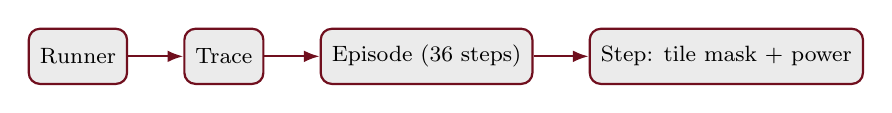
\begin{tikzpicture}
  \node[boxstyle] (v) {Runner};
  \node[boxstyle, right=7mm of v] (t) {Trace};
  \node[boxstyle, right=7mm of t] (e) {Episode (36 steps)};
  \node[boxstyle, right=7mm of e] (s) {Step: tile mask + power};
  \draw[arrowstyle] (v) -- (t);
  \draw[arrowstyle] (t) -- (e);
  \draw[arrowstyle] (e) -- (s);
\end{tikzpicture}
\end{center}
\note{Trace = viewing session, not video. The 3 validation traces are reused every checkpoint -- not an independent test set yet.}
\end{frame}

% --- time structure ---
\begin{frame}
\begin{itemize}
  \item Runner: 1{,}080 frames, 30 fps. GOP = 30 frames = 1 s.
  \item Step = 1 GOP. Episode = 36 steps.
  \item Rollout = 2{,}048 steps $\approx$ 56--57 episodes.
  \item PPO update: once per rollout.
  \item 700K run: 342 rollouts, 700{,}416 steps.
\end{itemize}

\vspace{10pt}
\begin{center}\small
\begin{tabular}{r c l}
36 steps & $\Rightarrow$ & 1 episode \\[4pt]
$\approx$56--57 episodes & $\Rightarrow$ & 1 rollout (2{,}048 steps) \\[4pt]
342 rollouts & $\Rightarrow$ & 700{,}416-step run \\
\end{tabular}
\end{center}
\note{700K = decisions, not episodes. Same video replayed many times over different traces and fresh channel draws.}
\end{frame}

% --- constraint budgets ---
\begin{frame}
\begin{itemize}
  \item Initial guidance (qualitative only, no numbers): power $\le$ UAV battery (no spec exists); tiles $\ge$ viewport size; stall budget to be swept.
  \item No numbers given $\to$ derived experimentally: \texttt{experiments/constraint\_calibration.py}.
  \item Method: exact $J_D,J_P,J_B$ ($\lambda=0.01$), 3 reference tile policies $\times$ 3 power levels, 9 training traces only, fixed seeds.
\end{itemize}

\vspace{8pt}
\begin{center}
{\footnotesize
\begin{tabular}{p{1.5cm}p{5.8cm}p{2.6cm}c}
\toprule
Budget & Finding & Reasoning & Chosen \\
\midrule
$\Dbar$ & efficient $J_D\approx0.00$; wasteful $J_D\approx0.60$ & inside range, near efficient end & $\mathbf{0.10}$ \\
$\Pbar$ & $J_P$ set by power level only: $0.00/0.505/1.01$ at min/mid/max & just above mid-power floor & $\mathbf{0.60}$ \\
$\Bbar$ & efficient $J_B\approx0.23$; wasteful $J_B\approx1.01$ & margin above mandatory floor & $\mathbf{0.35}$ \\
\bottomrule
\end{tabular}}
\end{center}
\note{P-bar needed different logic than D-bar/B-bar: J_P depends only on power level, not tile policy -- efficient-vs-wasteful tile comparison is degenerate for P specifically. All three confirmed before going into config.py.}
\end{frame}

% --- constrained objective + Lagrangian reward ---
\begin{frame}
\[
\max_{\pi}\ J_Q \qquad \text{s.t.} \qquad J_D\le\Dbar,\quad J_P\le\Pbar,\quad J_B\le\Bbar
\]
\[
r_{\mathrm{L}}^t \;=\; \beta_q\,\bar Q_{\mathrm{viewport}}^t \;-\; \mu_D\,\frac{D^t}{T_0} \;-\; \mu_P\,\frac{P^t}{P_{\max}} \;-\; \mu_B\,\frac{\sum_{i=1}^{N}x_i^t}{N}
\]
\begin{itemize}
  \item $\beta_q$ fixed. $\mu_D,\mu_P,\mu_B$ adaptive.
  \item $\Dbar,\Pbar,\Bbar$ not in this formula -- only in the multiplier update.
\end{itemize}
\note{Larger mu_j = stronger penalty for violating constraint j. Multipliers update once per rollout from that rollout's completed-episode costs, not every episode -- covered again on the training-loop slide.}
\end{frame}

% --- discount factor ---
\begin{frame}
\[
\lambda = 0.01, \qquad J_c = \sum_{t=0}^{35} \lambda^t c^t
\]
\begin{itemize}
  \item Weights: step 1 $=1$, step 2 $=0.01$, step 3 $=0.0001$.
  \item Applies to $J_Q,J_D,J_P,J_B$ -- same $\lambda$, same 36-step sum, every rollout.
\end{itemize}
\note{Only the first two steps matter numerically at this lambda -- everything past step 2 is under 0.01 percent weight. This is why J_Q stays near 1 regardless of whole-episode coverage.}
\end{frame}

% --- observation normalization ---
\begin{frame}
\[
\omega^t = \bigl[\,Z^t,\ \Delta_\theta^{t-1},\ \Delta_\phi^{t-1},\ h^t\,\bigr]
\]
\[
\hat\omega = \operatorname{clip}\!\left(\frac{\omega-\mu_{\mathrm{obs}}}{\sqrt{\sigma_{\mathrm{obs}}^2+\epsilon}},\,-10,\,10\right)
\]
\begin{itemize}
  \item \texttt{VecNormalize} (SB3): running mean/variance, training traces only.
  \item Frozen at validation. Checkpoint + \texttt{vecnormalize.pkl} always paired.
  \item Base-layer volume here: $\approx4.41$ Mbit/GOP. Reference paper: $A_{\text{base}}=4.5$ Mb.
\end{itemize}
\note{Why not the reference paper's fixed constants: our dataset-derived quantities differ from theirs, so an adaptive normalizer was used instead of borrowing their numbers.}
\end{frame}

% --- training / validation / checkpoint selection ---
\begin{frame}
\textbf{Per rollout:}
\begin{enumerate}
  \item Collect 2{,}048-step rollout.
  \item Update $\mu_D,\mu_P,\mu_B$ (rollout-averaged costs), then PPO parameter update.
  \item Evaluate on all 3 validation traces -- fixed seed per trace, frozen normalization.
  \item Save checkpoint + \texttt{vecnormalize.pkl} if new best.
\end{enumerate}

\vspace{8pt}
3 episodes $\times$ 36 steps $=$ 108 validation steps/event. Runs every rollout, not every 20K steps.

\vspace{8pt}
\textbf{Checkpoint selection:}
\begin{enumerate}
  \item Keep checkpoints with $J_D\le\Dbar$, $J_P\le\Pbar$, $J_B\le\Bbar$.
  \item Among feasible: highest $J_Q$.
  \item None feasible: smallest violation.
\end{enumerate}

\vspace{8pt}
\footnotesize Violation logged $=\sum_j\max(0,J_j-\bar b_j)$ -- raw sum, not scaled by budget size.
\note{Flag the raw-sum violation naming as something to fix later, not a hidden bug. Validation cadence upgraded from the original 20K-step plan to every rollout since it is cheap: 108 steps vs. 2048.}
\end{frame}

% --- results: 50K / 300K / 700K progression ---
\begin{frame}
\begin{center}
{\scriptsize
\setlength{\tabcolsep}{4pt}
\begin{tabular}{lccc}
\toprule
Validation & $\approx$51.2K & $\approx$301K & 700{,}416 (final) \\
\midrule
Feasible & 0 & 0 & \textbf{1} \\
$J_D$ ($\le0.10$) & 0.2755 & 0.1379 & 0.0000 \\
$J_P$ ($\le0.60$) & 0.2525 & 0.2525 & 0.2525 \\
$J_B$ ($\le0.35$) & 0.4840 & 0.4051 & 0.1898 \\
$J_Q$ & 1.0073 & 1.0073 & 1.0066 \\
Violation & 0.3095 & 0.0930 & \textbf{0.0000} \\
Coverage & 0.904 & 0.858 & 0.840 \\
Stall (s) & 0.391 & 0.169 & 0.001 \\
Power (mW) & 25 & 25 & 25 \\
Enh. tiles & 35.7 & 25.0 & 17.0 \\
\bottomrule
\end{tabular}}
\end{center}
\vspace{6pt}
\footnotesize Checkpoint near 294{,}912 steps: violation $\approx0.0569$ (better than that run's own final). 700K run: 342 rollouts, 140/342 feasible, last 20/20 feasible.
\note{All validation metrics, not training. Infeasible at 50K, closer at 300K, sustained feasible at 700K. Final checkpoint is not always the best checkpoint -- the 294,912-step example shows this directly.}
\end{frame}

% --- results: final behavior and trade-offs ---
\begin{frame}
\begin{center}
{\footnotesize
\begin{tabular}{lcc}
\toprule
 & Start & End \\
\midrule
\multicolumn{3}{l}{\textit{Physical (training)}} \\
Stall (s) & 0.531 & 0.022 \\
Enh. tiles & 39.1 & 19.0 \\
Power (mW) & 49.6 & 27.6 \\
Coverage & 0.927 & 0.882 \\
\addlinespace
\multicolumn{3}{l}{\textit{Multipliers}} \\
$\mu_D$ & 1.00 & 1.71 \\
$\mu_B$ & 1.00 & 1.46 \\
$\mu_P$ & 1.00 & 0.009 \\
\addlinespace
\multicolumn{3}{l}{\textit{Training diagnostic}} \\
Explained var. & $\approx0$ & 0.41 \\
\bottomrule
\end{tabular}}
\end{center}
\vspace{6pt}
\begin{itemize}\footnotesize
  \item 19.0 enhanced tiles = mandatory (predicted viewport) + agent-chosen extra -- not 19 agent-picked tiles alone.
  \item $\mu_P\to0.009$: power constraint slack at $\Pbar=0.6$.
\end{itemize}
\note{Stall and tiles down a lot, coverage down a little -- a real trade-off, not noise. 0.022s stall is very low, not exactly zero. Do not call multiplier stability alone convergence -- sustained feasibility is the stronger evidence.}
\end{frame}

% --- results: power action, deeper look ---
\begin{frame}
\begin{itemize}
  \item Discrete power levels: 0/25/50/75/100 mW (5 levels).
  \item Trained policy (best \& final checkpoint): \textbf{100\% of steps $\to$ level 1 (25 mW)}. Zero variation across buffer level, prediction error, channel gain.
  \item $J_P$ at level 1 $\approx0.2525$ vs.\ budget $\Pbar=0.6$ -- large margin.
  \item Tiles: mandatory (predicted viewport) mean $\approx14$ of 64 (range 9--16). Agent's own extra tiles: best checkpoint $\approx6.6$, final checkpoint $\approx3.0$.
\end{itemize}
\vspace{6pt}
\footnotesize Policy never differentiates power by state. Consistent with $\mu_P\to0$: no reward pressure to go higher or lower once level 1 avoids stalling.
\note{This is the evidence behind changing the power action space: 5 levels across the full 0-100 percent range, but the policy only ever uses the second-lowest one. A narrower range, e.g. 0-50 percent, still 5 slots, would give resolution where the policy actually operates.}
\end{frame}

% --- questions ---
\begin{frame}
\begin{itemize}
  \item Keep $\lambda=0.01$, or change it?
  \item How many total steps to train -- is 700K enough, or keep going?
  \item Are these the right evaluation metrics?
  \item Move next to comparing PPO vs.\ PPO + PDS + VE?
  \item Change $\Pbar$, given $\mu_P\to0$ (power not binding)?
  \item Change the power action space -- narrower range (e.g.\ 0--50\%) with the same 5 slots, for finer resolution where the policy actually operates?
\end{itemize}
\note{Prioritize the P-bar / power-action-space question and the training-length question if time is short.}
\end{frame}

\end{document}
